\section{Forward Simulation Examples}

When a generic disease model is initialized with all-cause mortality
data and nothing else, the initial values produce the following set of
consistent age patterns:

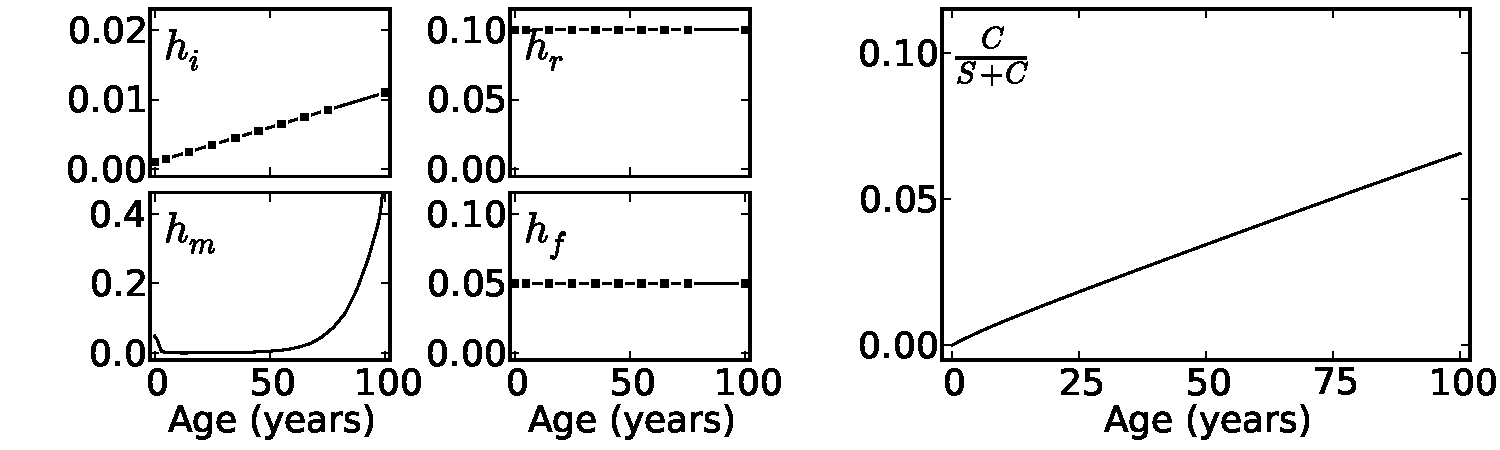
\includegraphics[width=\textwidth]{initial.png}

The next example shows that increasing the remission rate with
incidence and excess mortality unchanged (and all-cause mortality
unchanged as well) leads to a very different age pattern for
prevalence. It is also worth pointing out that since prevalence has
changed with excess mortality and all-cause mortality rates held
constant, the with-condition and background mortality rates have also
changed to maintain consistency.

\includegraphics[width=\textwidth]{more-remission.png}

By changing the incidence rate age pattern to be increasing as a
function of the square root age, I can demonstrate that very similar
prevalence rates are consistent with very different incidence and
remission rates.

\includegraphics[width=\textwidth]{increasing-incidence.png}

Although the prevalence age pattern is largely determined by the
remission, incidence, and mortality rates, the birth prevalence can
also change the shape dramatically.  Here are the results of the same
remission, incidence, and mortality rates as above, but with a birth
prevalence of 20\%.

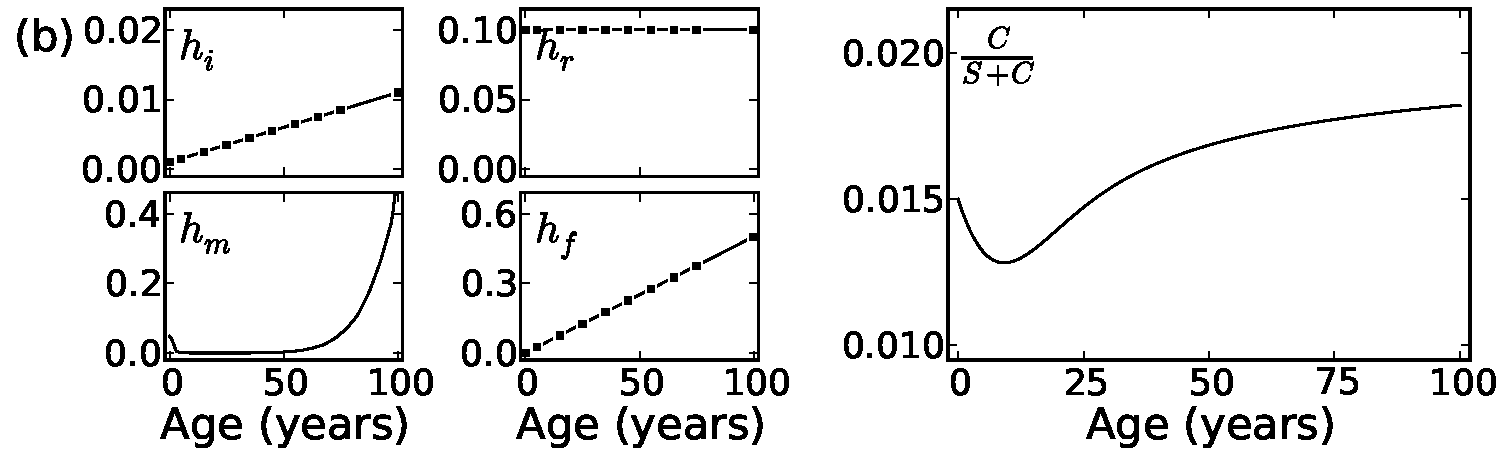
\includegraphics[width=\textwidth]{birth-prevalence.png}

An interesting, and perhaps unexpected feature of this set of
consistent rates above is that when prevalence levels start so high,
the levels remain high during the teenage years, where all-cause
mortality rates are quite low in this population (following the rates
for males in the North American High Income region in 2005), which
produces very low levels of background mortality for these age
groups. In other words, in order for the model to be consistent, it is
necessary to assume that the vast preponderance of teenage deaths are
due to this disease.

Finally, the excess mortality rate (which is the most difficult of the
rates to conceptualize, due to its unobservability) has an effect of
modulating the prevalence that is similar to the remission rate,
although not identical.  The final figure in this series shows the
results of choosing an excess mortality rate to have an age function
equal to ten times the all-cause mortality rate (which is to say a
standardized mortality rate of constant value eleven for all ages).

\includegraphics[width=\textwidth]{higher-smr.png}

The decreasing prevalence after age 65 is worthy of remarking
on. Although the incidence rate is increasing and the remission rate
remains unchanged, having a constant (albeit high) standardized
mortality ratio means that when all-cause mortality rises, the
with-condition mortality rises differentially with such magnitude that
the prevalence of the condition in older populations goes down.

To summarize, this series of figures has shown the intuitive and
less-than-intuitive way that the levels and age patterns of different
epidemiological parameters must be interrelated to satisfy the
fundamental equations of population health (when disease rates for
each age are changing negligibly slowly as a function of time).

The next series of figures continues to build familiarity with the
features of consistent disease modeling, by selecting age patterns for
certain rates based on toy models of a variety of diseases.  For
example, for a disorder like depression, for which there is primarily
incidence in early adulthood, high remission rate, and low excess
mortality, the consistency conditions produce a prevalence age pettern
that peaks at age 25: 

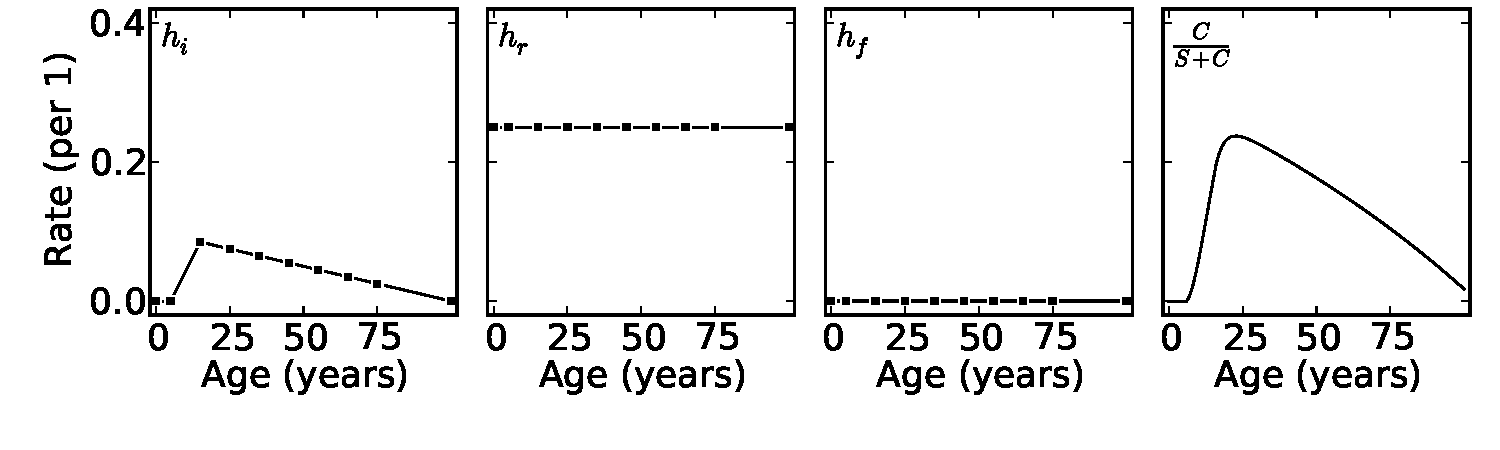
\includegraphics[width=\textwidth]{forward-sim-mental.png}

For a congenital disorder, like TK, with birth prevalence, no
incidence after birth, no remission, and substantial mortality, the
consistent prevalence age pattern is the following:

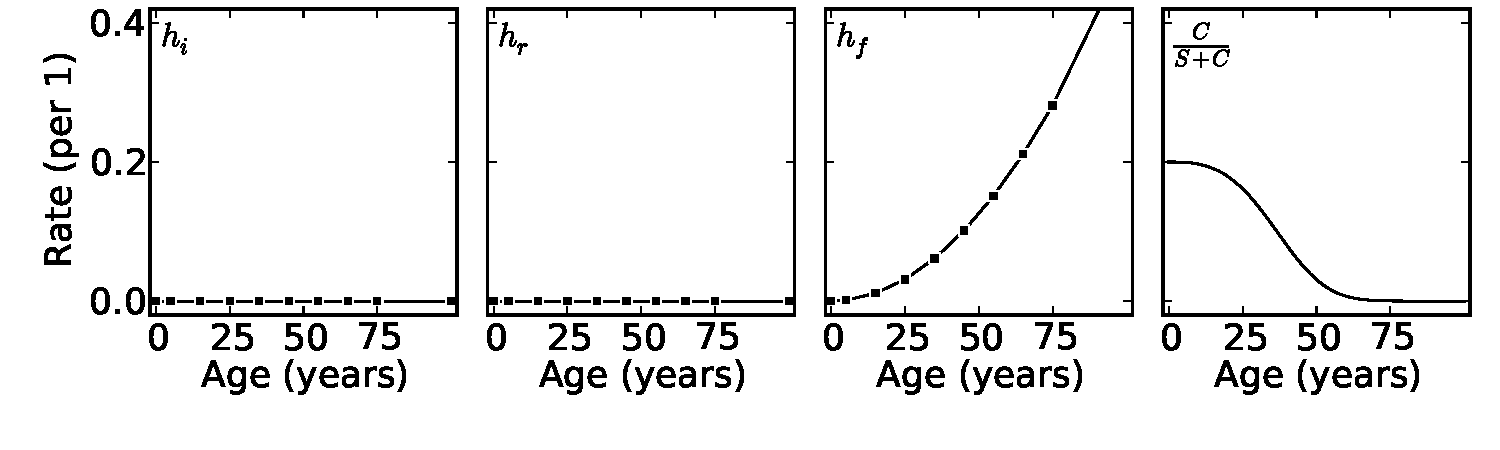
\includegraphics[width=\textwidth]{forward-sim-congenital.png}

For a disorder that affects the elderly, like TK, the consistent age
patterns for mortality, incidence, remission, and prevalence could
look like the following: 

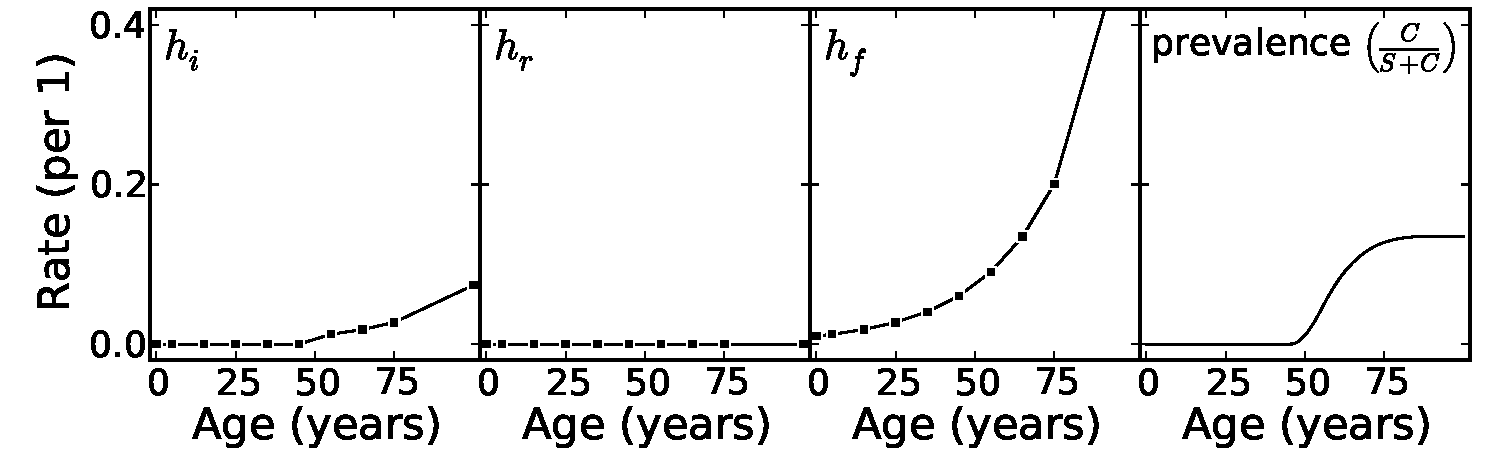
\includegraphics[width=\textwidth]{forward-sim-old_age.png}

And for a disorder related to the reproductive system, like TK, with
substantial excess mortality and incidence during ages 15-60, and
remission that increases substantially at age 55, the consistent age
patterns could look like the following: 

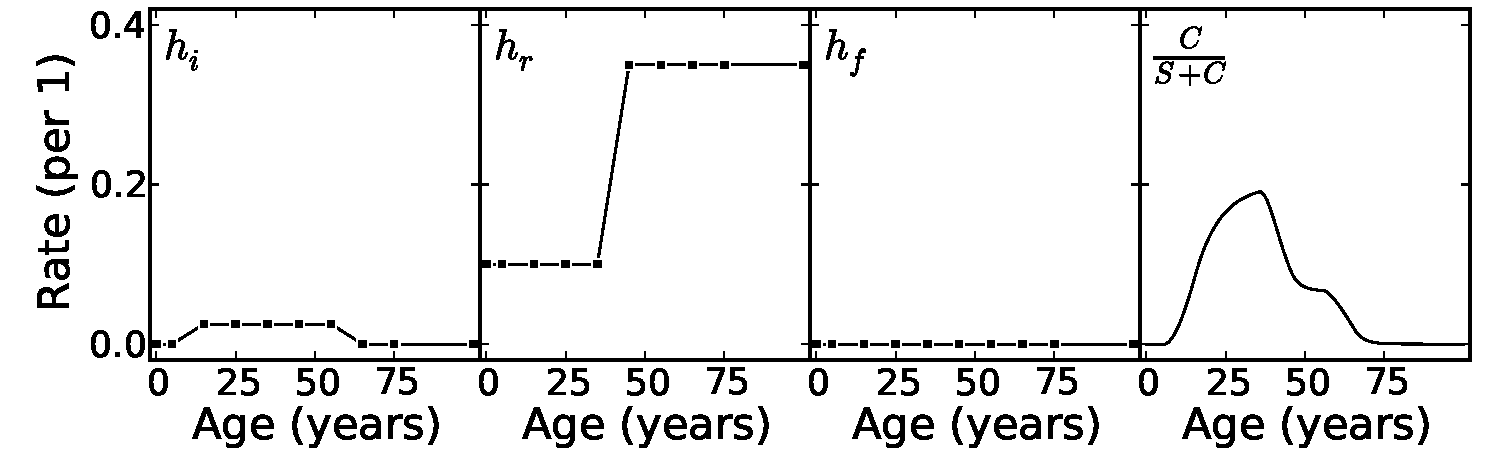
\includegraphics[width=\textwidth]{forward-sim-reproductive.png}

To conclude this series of plots, I've included an "incidence impulse
response" example, showing the prevalence produced to be consistent
with an incidence pattern that is only nonzero for a single age group:

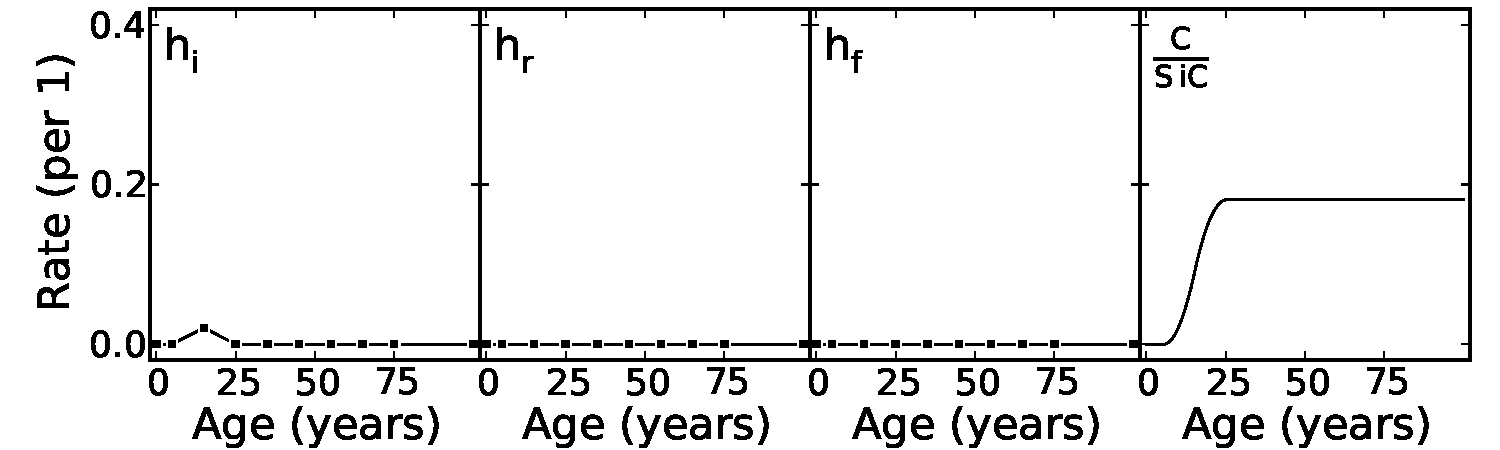
\includegraphics[width=\textwidth]{forward-sim-incidence_pulse.png}

This also provides a mechanism to investigate how wrong the estimates
may become when the assumption that rates are constant over time (for
a given age) is violated. This is the core of my simulation approach
to model validation, to which I will return in section TK.

TK The simulation study approach can be described in full detail here
as well, and can serve as justification for decisions described in the
next two chapters.

\section{What happens to prevalence when the disease incidence or remission or mortality is not constant over time?}

Certain important diseases such as diabetes are widely believed to
have substantial changes in incidence, remission, and mortality rates
over time.  What is the effect of the endemic equilibrium assumption
of the age-specific prevalence. TK plots comparing prevalence from a
synthetic cohort model to a period model using simulation data.
